\documentclass[12pt,pdftex,a4paper]{article}
\usepackage[english]{babel}
\usepackage{enumitem} 
\usepackage{amsmath}
\usepackage{amssymb}
\usepackage{bbm}
\usepackage[utf8]{inputenc}
\usepackage{float}
\usepackage{cleveref}

\newcommand{\bbN}{\mathbbm{N}}
\newcommand{\bbR}{\mathbbm{R}}
\newcommand{\bbZ}{\mathbbm{Z}}
\newcommand{\bbI}{\mathbbm{I}}

\usepackage{amsthm}
\usepackage{amsfonts}

\usepackage{mathtools}
\usepackage{esvect} % Schöne Vektorpfeile mit \vv{\alpha}
\usepackage[usenames]{color}
\usepackage{polynom}
\usepackage{geometry}
\usepackage{tikz}
\usetikzlibrary{decorations.pathreplacing}
\geometry{verbose,a4paper,tmargin=25mm,bmargin=25mm,lmargin=15mm,rmargin=15mm}
\usepackage{graphicx}
\makeatletter
\def\ScaleIfNeeded{%
\ifdim\Gin@nat@width>\linewidth
\linewidth
\else
\Gin@nat@width
\fi
}
\makeatother

%\geometry{verbose,a4paper,tmargin=25mm,bmargin=25mm,lmargin=15mm,rmargin=20mm}
 
\title{Mathe}

\newcommand{\setN}[0]{\mathbb{N}}
\newcommand{\setF}[0]{\mathbb{F}}
\newcommand{\setR}[0]{\mathbb{R}}
\newcommand{\setZ}[0]{\mathbb{Z}}
\newcommand{\setC}[0]{\mathbb{C}}
\newcommand{\setP}[0]{\mathbb{P}}
\newcommand{\setQ}[0]{\mathbb{Q}}
\newcommand{\setK}[0]{\mathbb{K}}
\newcommand{\winkel}{<\hspace{-1.25ex})\hspace{2.25ex}}
\newcommand{\axi}[1]{{\label{#1}(#1)}}
\newtheorem{defi}{Definition}[section]
\newtheorem{satz}[defi]{Satz}
\newtheorem{prop}[defi]{Proposition}
\newtheorem{koro}[defi]{Korollar}
\newtheorem{lemma}[defi]{Lemma}
\newtheorem*{bsp}{Beispiel}
\newtheorem*{commen}{Bemerkung}
\newenvironment{alphb}{\begin{enumerate}
\def\theenumi{(\alph{enumi})}}{\end{enumerate}}
\newenvironment{arabb}{\begin{enumerate}
\def\theenumi{\arabic{enumi})}}{\end{enumerate}}
\renewcommand{\labelenumi}{\theenumi}
\renewcommand{\theenumi}{\arabic{enumi}.}
\newcommand{\litoinf}{\lim\limits_{n\to\infty}}
\newcommand{\sumtoinf}{\sum\limits_{n=0}^\infty}
\newcommand{\sumtok}{\sum\limits_{n=0}^k}
\newcommand{\sumin}{\sum\limits^\infty}
\newcommand{\fol}{_{n\in\setN}}
\newcommand{\dx}{\mathrm{d}x}
\newcommand{\dt}{\mathrm{d}t}
\usepackage{tabulary}
\usepackage{pdfpages}
\DeclareMathOperator{\Span}{Span}
\let\oldphi\phi
\renewcommand \phi \varphi
\newcommand \my \mu
\definecolor{dunkelgruen}{rgb}{0,0.4,0}


%\usepackage[pdftex]{graphicx}
\usepackage{listings}
\lstset{language=Python,basicstyle=\footnotesize}

\usepackage{newunicodechar}
\newunicodechar{°}{\deg} % \deg wird zum °-Zeichen für Winkel oder Temperaturen. kA, warum LaTeX das nicht direkt mag.
\begin{document}
\title{Bachelor-Forschungsprojekt Informatik:\\Relevante OSM-Tags vorschlagen}
\author{Marco Hildebrand, XXXX, stXXXX@stud.uni-stuttgart.de\\
		Lukas Baur, 3131138, st141998@stud.uni-stuttgart.de\\
		Felix Bühler, 2973410, st117123@stud.uni-stuttgart.de}
\maketitle

\section*{Abstract}
Die vom \textit{Institut für Formale Methoden der Informatik Stuttgart} entwickelte textbasierte Suchmaschine \textit{OSCAR}, die OpenStreetMap-Daten auf Eingabe von OSM-Tags durchsucht, liefert unbefriedigende Ergebnisse auf anderweitige textuelle Eingaben. 
Im Rahmen unseres Bachelor-Forschungsprojekt Informatik sollte diese Lücke geschlossen werden, indem eine Anfrage an das von uns entwickelte System eine Menge an damit verwandten, relevanten Tags zurückgibt.

\pagebreak

\section{Einleitendes}
\subsection{Projektrahmen}
Die Arbeit wurde im Rahmen des \textit{Bachelor-Forschungsprojekts Informatik} in der Zeit vom April bis Oktober 2018 angefertigt. Diese Ausarbeitung stellt die inhaltliche Dokumentation des entwickelten Moduls dar.
\subsection{Initiale Problemstellung}
Grundlage für unsere Arbeit war die Suchmaschine \textit{OSCAR}, die vom \textit{Institut für Formale Methoden der Universität Stuttgart} entwickelt wurde.\\
OSCAR durchsucht auf Eingabe eines \textit{OpenStreetMap-Tags} die  zugehörige Datenbank nach passenden Einträgen und bereitet das Suchresultat grafisch auf. Ein \textit{Tag} ist in OpenStreetMap wie folgt definiert:
\begin{center}
	\textbf{\textit{key}=\textit{value}}
\end{center}
Ein \textit{key} wird benutzt, um ein Themenbereich zu charakterisieren, es repräsentiert einen Typ oder beschreibt ein Feature. Außerdem werden Tags vereinzelt als Namespaces verwendet \cite{keyDescription}.\\
Der \textit{value}-Teil stellt ein Wert des Features da. Typische Werte sind Eigenschaften oder Zahlen \cite{keyDescription}.
Beispiele für Tags sind \textit{building=yes}, \textit{building=house} oder  \textit{highway=service} \cite{example1}\cite{example2}.\\

Da die Eingabe auf Tags beschränkt ist, benötigt ein User zur Suche einen passenden Tag. Diese Lücke soll mithilfe dieses Projekts geschlossen werden. Das zu entwickelnde System soll auf Eingabe eines natürlichen Wortes der englischen Sprache möglichst eng verwandte, relevante OpenStreetMap-Tags vorschlagen.

\subsection{Abgrenzungen}
Unsere Arbeit konzentriert sich auf die Suche der relevanten Tags zu einem eingegebenen Wort. Formaler ausgedrückt besteht unsere Eingabe aus genau einem Wort der englischen Sprache, das nicht in der zugrundeliegenden Stop-Word-Liste enthalten ist.


\section{Projekt-Durchführung}
\subsection{Planungsaspekte}
Zu Beginn unserer Arbeit grenzten wir unser Projekt thematisch ein und überlegten uns eine grobe Vorstrukturierung.
Dazu gliederten wir unser Projekt in \textbf{drei} wesentliche Bausteine:\\
Im zeitlich ersten Arbeitsblock sollten wir uns mit der Darstellung, der Qualität und der Möglichkeit des Zugriffs der Daten vertraut machen. Im Folgenden überlegten wir uns eine aufbereitete brauchbare Daten-Zwischenform, auf deren Grundlage die spätere Suche durchgeführt werden soll. Der dritte Arbeitsbaustein galt der eigentlichen Such-Implementierung.\\
Die bearbeiteten Arbeitspakete werden im folgenden inhaltlich beschrieben. Die Pakete sind intern zeitlich sequentiell beschrieben, überlappen sich allerdings in Ihrer Abarbeitung. Der Grund hierfür sind Abhängigkeiten, wie zum Beispiel, dass die Datenaufbereitung an die Repräsentation des Suchalgorithmus angepasst werden muss, zuvor aber Daten als Grundlage der Suche beschafft sein müssen.

\subsection{Datenbeschaffung}
Unsere anfängliche Recherche begannen wir mit der Website von OpenStreetMap \cite{WebsiteOSM}, insbesondere mit dem zugehörigem Wiki \cite{WebsiteOSMWiki}. Das OSM-Wiki verfügt über eine ausführliche Dokumentation vieler gängiger OSM-Tags. Unser Ziel war es, auf alle vorhandenen Daten-Tupel, bestehend aus einem gültigen Tag und einer zugehörigen Tag-Beschreibung, lokalen Zugriff zu haben.
\\
Leider besteht keine Möglichkeit das OSM-Wiki herunter zu laden. Wir kontaktierten den Verantwortlichen des Wikis, dieser konnte uns allerdings ebenfalls keine Kopie zukommen lassen. Folglich müssten wir die Webseiten des Wikis automatisiert crawlen. 
\\
Zwischenzeitlich versuchten wir alternativ mithilfe der Website \textit{taginfo} \cite{taginfoWebsite} an die gesuchten Daten zu gelangen. taginfo wurde in Zusammenarbeit von Jochen und Christian Topf entwickelt und sammelt auf Grundlage der OSM-Daten aktuell rund 2.500 Tags inklusive deren statistischen Charakteristika und teilweise Beschreibungen\cite{taginfoAbout}. Zusätzlich besteht die Möglichkeit, die komplette Datenbank herunterzuladen.\\
\begin{figure}[h]
	\centering
	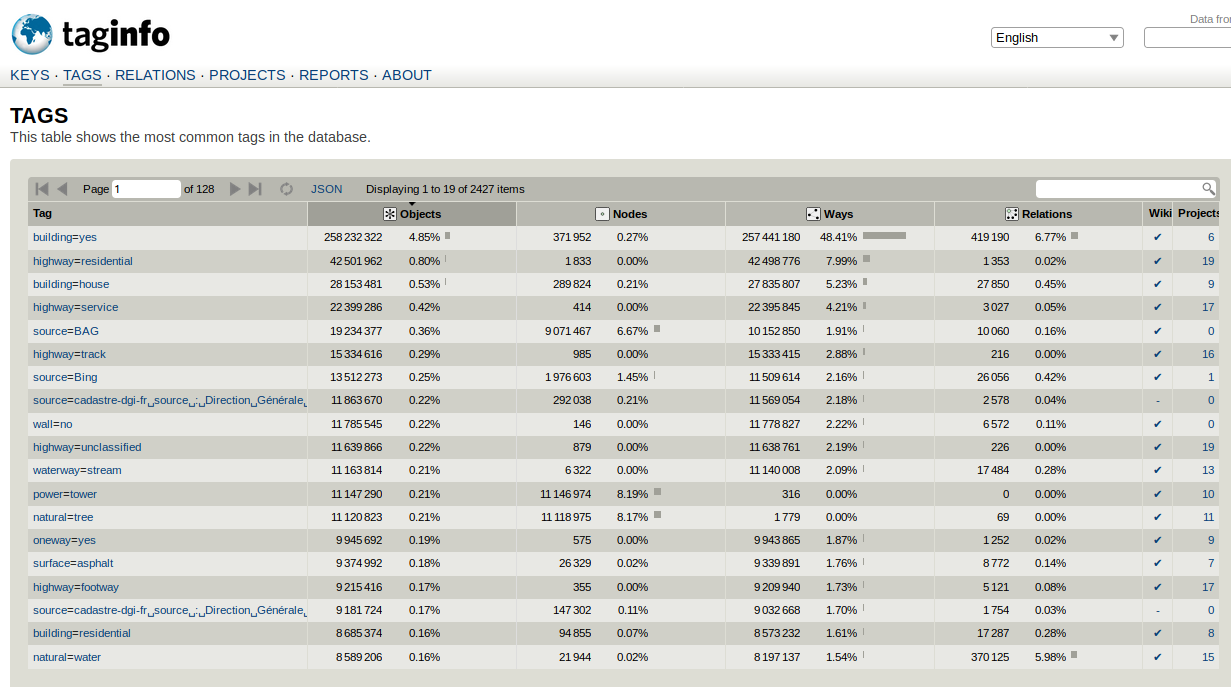
\includegraphics[width=0.9\linewidth]{Bilder/taginfo_example}
	\caption[Beispielhafte Darstellung taginfo]{Beispielhafte Datenbankeinträge der Datenbank von taginfo}
	\label{fig:taginfoexample}
\end{figure}

Leider stellten wir fest, dass die Beschreibungs-Einträge der Datenbank zu lückenhaft und damit für unsere Zwecke nicht geeignet sind.
Schließlich kombinierten wir unsere bisherigen Ansätze, indem wir die Tag-Einträge der heruntergeladenen taginfo-Datenbank als Grundlage für ein Crawlen der OSM-Wiki-Seite verwendeten. Dies war möglich, da neben der lückenhaften Beschreibung zu jedem Tag zusätzlich der Link zur Wiki-Seite abgespeichert war. Dieser generische Link bestand aus den Teilen
\begin{center}
	\textbf{wiki.openstreetmap.org/wiki/Tag\%3\textit{Key}\%3D\textit{value}}
\end{center}
wobei die Variablen \textit{key} und \textit{value} gemäß obiger Erklärung zu füllen sind.



\subsection{Datenaufbereitung}

\subsection{Suchanfrage beantworten}

\section{notizen}
Phase 1: Planung
- Tags und dazugehörige semantische Beschreibung holen
- in Struktur bringen
- Suchanfrage an Daten 
    - gensim (Python von Mendel zu Beginn vorgeschlagen)
	- vorhanden/nicht vorhanden 
		-> bewerbung fehlt
	- tf-idf
		-> gut, aber Problem: Mehrere Links auf dieselbe Seite
			-> Duplikate entfernen
		-> hohe Gewichtung für kleine Seiten
			-> Multiplizieren mit log/oder Wurzel 2
- Suchraum expandieren
	- mit Google Modell Anfrage semantisch auffüllen, Suche durchführen, am meisten Relevanten herausnehmen.

\section{Einleitung}
\subsection{Projektbeschreibung}

\pagebreak
\section{Vorgehensweise}
Anschauen von wiki xml dump

unbrauchbare daten, da viel untereinander verlinkt ist.

herunterladen der tags: https://taginfo.openstreetmap.org/

\section{Gettings started}
\subsection{languages}
einfach eine liste aller sprachen bekommen mithilfe \texttt{taginfo-wiki.db}.

Die kann man von \texttt{https://taginfo.openstreetmap.org/download} herunterladen.

\subsection{export-links}
herunterladen der osm-wiki sitemap
\texttt{https://wiki.openstreetmap.org/sitemap-index-wiki.xml}


davon interessiert uns nur \texttt{sitemap-wiki-NS\_0-0.xml} der rest enthält daten zu den nutzern, diskussionen und historie

\section{crawl}
alle gesammelten link in die \texttt{links.txt} legen

\texttt{scrapy crawl osmWiki -t json -o keys.json}

\subsection{pretty json}
\texttt{python -m json.tool keys.json > keys-pretty.json}


\pagebreak
\section{Anhang}


\bibliographystyle{unsrt}
\bibliography{lit}

\end{document}
